\section{Controls and robustness}

The controls change only one thing: the exact string scored after ``\texttt{Final answer:}''.
Figure~\ref{fig:controls} shows why that matters. Under identity ordering, the primary
exact-option readout yields a \SemanticIdentityValidRate{} valid-rate for
$\Delta_{\mathrm{margin}}$. If we keep the prompt fixed but score the literal continuation
``\texttt{The answer is \{option\}}'' instead, that valid-rate falls to
\TemplatedIdentityValidRate{}. If we score only the answer letter, it rises to
\LetterIdentityValidRate{}.

The broad phenomenon does persist under both controls. On the fully paired identity subset,
the median lag is \SemanticPairedLagMedian{} layers for the exact-option readout,
\TemplatedPairedLagMedian{} layers for the templated control, and
\LetterPairedLagMedian{} layers for the letter-label control. The share of positive-lag cases
on that same paired subset is \SemanticPairedPositivePct{}, \TemplatedPairedPositivePct{},
and \LetterPairedPositivePct{}, respectively. So the main effect is not unique to one answer
format.

\begin{figure}[t]
\centering
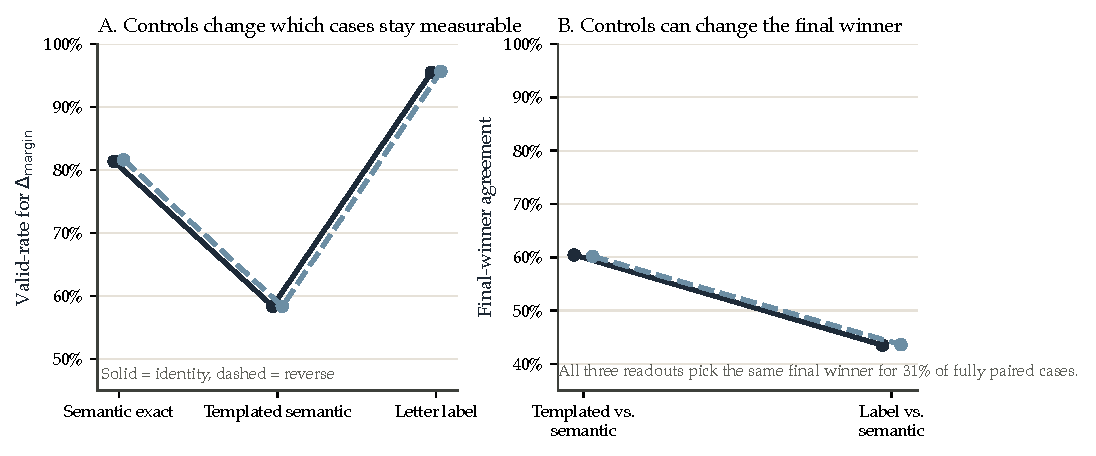
\includegraphics[width=\columnwidth]{figure3_control_readout_comparison.pdf}
\caption{\textbf{The broad lag survives the controls, but the controls still change the measurement.} Panel A shows how often $\Delta_{\mathrm{margin}}$ is defined for each readout. Panel B shows how often the two control readouts pick the same final winner as the semantic-exact primary readout on fully paired cases. Identity and reverse order behave similarly. The answer-format controls do not, which is why they are useful robustness checks but not replacements for the main semantic path.}
\label{fig:controls}
\end{figure}

The readouts also disagree on which answer the model prefers at the end. In fully paired
identity cases, the templated control agrees with the exact-option path on only
\TemplatedAgreementIdentity{} of cases, the letter-label control agrees on only
\LetterAgreementIdentity{}, and all three readouts agree on just \AllSameReadoutRate{} of
cases. This is exactly why we kept the controls. They tell us that the early-candidate /
late-commitment pattern is fairly robust, while also showing that different answer formats
can change the evaluable set and can even change the final winner. That makes the controls
scientifically useful, but it also means they are not interchangeable with the primary
exact-option analysis.

The answer-order control tells a different story. In Figure~\ref{fig:controls}, the identity
and reverse traces are nearly on top of each other. That is reassuring because it suggests
the main effect is not coming from one arbitrary option order. The report-only robustness
summaries also line up with the primary rule. The secondary criterion yields the same
positive pattern as the primary rule (\OverallSecondaryPositiveCells{} positive,
\OverallSecondaryInsufficientCells{} insufficient), and the gold-answer sensitivity analysis is
positive on all \GoldArcCsqaPositiveCells{} evaluable ARC-Challenge and CommonsenseQA
cells.

Finally, the QC path is designed to surface problems, not hide them. The released audit bundle logs \TokenCollisionCount{} tokenization collisions and \DuplicateOptionCount{} duplicate-option examples instead of silently dropping them, while the merged run itself still has zero failure rows and zero unpaired rows. The point is not to make the result look tidy. The point is to show that the result still holds when we keep the pipeline honest about edge cases.

\FloatBarrier
